%package list
\documentclass{article}
\usepackage[top=3cm, bottom=3cm, outer=3cm, inner=3cm]{geometry}
\usepackage{multicol}
\usepackage{graphicx}
\usepackage{url}
%\usepackage{cite}
\usepackage{hyperref}
\usepackage{array}
%\usepackage{multicol}
\newcolumntype{x}[1]{>{\centering\arraybackslash\hspace{0pt}}p{#1}}
\usepackage{natbib}
\usepackage{pdfpages}
\usepackage{multirow}    
\usepackage[normalem]{ulem}
\useunder{\uline}{\ul}{}
\usepackage{svg}
\usepackage{xcolor}
\usepackage{listings}
\lstdefinestyle{ascii-tree}{
    literate={├}{|}1 {─}{--}1 {└}{+}1 
  }

\lstset{basicstyle=\ttfamily,
  showstringspaces=false,
  commentstyle=\color{red},
  keywordstyle=\color{blue}
}
%\usepackage{booktabs}
\usepackage{caption}
\usepackage{subcaption}
\usepackage{float}
\usepackage{array}

\usepackage{enumitem}


\newcolumntype{M}[1]{>{\centering\arraybackslash}m{#1}}
\newcolumntype{N}{@{}m{0pt}@{}}


%%%%%%%%%%%%%%%%%%%%%%%%%%%%%%%%%%%%%%%%%%%%%%%%%%%%%%%%%%%%%%%%%%%%%%%%%%%%
%%%%%%%%%%%%%%%%%%%%%%%%%%%%%%%%%%%%%%%%%%%%%%%%%%%%%%%%%%%%%%%%%%%%%%%%%%%%
\newcommand{\itemEmail}{}
\newcommand{\itemStudent}{Victor Gonzalo Maldonado Vilca, Armando Steven Cuno Cahuari}
\newcommand{\itemCourse}{ Estructura de Datos y Algoritmos (EDA) }
\newcommand{\itemCourseCode}{1702122}
\newcommand{\itemSemester}{III}
\newcommand{\itemUniversity}{Universidad Nacional de San Agustín de Arequipa}
\newcommand{\itemFaculty}{Facultad de Ingeniería de Producción y Servicios}
\newcommand{\itemDepartment}{Departamento Académico de Ingeniería de Sistemas e Informática}
\newcommand{\itemSchool}{Escuela Profesional de Ingeniería de Sistemas}
\newcommand{\itemAcademic}{2024 - A}
\newcommand{\itemInput}{ Del 13/06/2024}
\newcommand{\itemOutput}{ Al 13/06/2024 - 23:59pm}
\newcommand{\itemPracticeNumber}{05}
\newcommand{\itemTheme}{Adelson-Velskii y Landis (AVL)}
%%%%%%%%%%%%%%%%%%%%%%%%%%%%%%%%%%%%%%%%%%%%%%%%%%%%%%%%%%%%%%%%%%%%%%%%%%%%
%%%%%%%%%%%%%%%%%%%%%%%%%%%%%%%%%%%%%%%%%%%%%%%%%%%%%%%%%%%%%%%%%%%%%%%%%%%%

\usepackage[english,spanish]{babel}
\usepackage[utf8]{inputenc}
\AtBeginDocument{\selectlanguage{spanish}}
\renewcommand{\figurename}{Figura}
\renewcommand{\refname}{Referencias}
\renewcommand{\tablename}{Tabla} %esto no funciona cuando se usa babel
\AtBeginDocument{%
	\renewcommand\tablename{Tabla}
}

\usepackage{fancyhdr}
\pagestyle{fancy}
\fancyhf{}
\setlength{\headheight}{30pt}
\renewcommand{\headrulewidth}{1pt}
\renewcommand{\footrulewidth}{1pt}
\fancyhead[L]{\raisebox{-0.2\height}{
\includegraphics[width=3cm]{img/logo_episunsa.png}}}
\fancyhead[C]{\fontsize{7}{7}\selectfont	\itemUniversity \\ \itemFaculty \\ \itemDepartment \\ \itemSchool \\ \textbf{\itemCourse}}
\fancyhead[R]{\raisebox{-0.2\height}{
\includegraphics[width=1.2cm]{img/logo_abet}}}
\fancyfoot[L]{Victor M.}
\fancyfoot[C]{\itemCourse}
\fancyfoot[R]{Página \thepage}

% para el codigo fuente
\usepackage{listings}
\usepackage{color, colortbl}
\definecolor{dkgreen}{rgb}{0,0.6,0}
\definecolor{gray}{rgb}{0.5,0.5,0.5}
\definecolor{mauve}{rgb}{0.58,0,0.82}
\definecolor{codebackground}{rgb}{0.95, 0.95, 0.92}
\definecolor{tablebackground}{rgb}{0.8, 0, 0}

\lstset{frame=tb,
	language=bash,
	aboveskip=3mm,
	belowskip=3mm,
	showstringspaces=false,
	columns=flexible,
	basicstyle={\small\ttfamily},
	numbers=none,
	numberstyle=\tiny\color{gray},
	keywordstyle=\color{blue},
	commentstyle=\color{dkgreen},
	stringstyle=\color{mauve},
	breaklines=true,
	breakatwhitespace=true,
	tabsize=3,
	backgroundcolor= \color{codebackground},
}

\begin{document}
	
	\vspace*{10px}
	
	\begin{center}	
		\fontsize{17}{17} \textbf{ Informe de Laboratorio 05}
	\end{center}
	\centerline{\textbf{\Large Tema: \itemTheme}}
	%\vspace*{0.5cm}	

	\begin{flushright}
		\begin{tabular}{|M{2.5cm}|N|}
			\hline 
			\rowcolor{tablebackground}
			\color{white} \textbf{Nota}  \\
			\hline 
			     \\[30pt]
			\hline 			
		\end{tabular}
	\end{flushright}	

	\begin{table}[H]
		\begin{tabular}{|x{4.7cm}|x{4.8cm}|x{4.8cm}|}
			\hline 
			\rowcolor{tablebackground}
			\color{white} \textbf{Estudiante} & \color{white}\textbf{Escuela}  & \color{white}\textbf{Asignatura}   \\
			\hline 
			{\itemStudent \par \itemEmail} & \itemSchool & {\itemCourse \par Semestre: \itemSemester \par Código: \itemCourseCode}     \\
			\hline 			
		\end{tabular}
	\end{table}		
	
	\begin{table}[H]
		\begin{tabular}{|x{4.7cm}|x{4.8cm}|x{4.8cm}|}
			\hline 
			\rowcolor{tablebackground}
			\color{white}\textbf{Tarea} & \color{white}\textbf{Tema}  & \color{white}\textbf{Duración}   \\
			\hline 
			\itemPracticeNumber & \itemTheme & 2 horas   \\
			\hline 
		\end{tabular}
	\end{table}
	
	\begin{table}[H]
		\begin{tabular}{|x{4.7cm}|x{4.8cm}|x{4.8cm}|}
			\hline 
			\rowcolor{tablebackground}
			\color{white}\textbf{Semestre académico} & \color{white}\textbf{Fecha de inicio}  & \color{white}\textbf{Fecha de entrega}   \\
			\hline 
			\itemAcademic & \itemInput &  \itemOutput  \\
			\hline 
		\end{tabular}
	\end{table}
%%%%%%%%%%%%%%%%%%%%

  \section{Introducción}
  Los árboles AVL son una estructura de datos de árbol binario de búsqueda auto-balanceado, nombrados en honor a sus inventores, 
  Georgy Adelson-Velsky y Evgenii Landis, quienes los introdujeron en 1962. Estos árboles se diseñaron para mantener un 
  equilibrio dinámico que garantiza que las operaciones de búsqueda, inserción y eliminación puedan realizarse en tiempo 
  logarítmico O(log n). Este equilibrio se logra mediante la restricción de la diferencia de altura (balanceo) entre los 
  subárboles izquierdo y derecho de cualquier nodo a un máximo de uno.

%%%%%%%%%%%%%%%%%%%%

  \section{Objetivos}
  \begin{itemize}
    \item Entender los conceptos básicos de los árboles AVL.
    \item Implementar correctamente las operaciones básicas.
    \item Mantener el equilibrio del árbol
    \item Optimizar el tiempo de búsqueda.
    \item Fomentar buenas prácticas de programación.
    \item Mejorar la eficiencia en la inserción y eliminación.
  \end{itemize}

%%%%%%%%%%%%%%%%%%%%
 
	\section{Tarea}
  Elabore un informe implementando Arboles AVL con toda la lista de operaciones(adapte el código de las diapositivas) : 
  \begin{itemize}
    \item search(),
    \item getMin(), 
    \item getMax(), 
    \item parent(), 
    \item son(), 
    \item insert()
  \end{itemize}
  \textbf{INPUT:} Una sóla palabra en mayúsculas.\newline
  \textbf{OUTPUT:} Se debe construir el  árbol AVL considerando el valor decimal de su código ascii.
  Luego, pruebe todas sus operaciones implementadas.\newline
  \textbf{Pregunta:}
  ¿Explique como es el algoritmo que implementó para obtener el factor de equilibrio de un nodo?
 
%%%%%%%%%%%%%%%%%%%% 
 
  \section{Entregables}
  \begin{itemize}
    \item Informe hecho en latex.
    \item Archivos java.
    \item Responder la pregunta dejada.
    \item URL: Repositorio GitHub.
  \end{itemize}
  
%%%%%%%%%%%%%%%%%%%%    
		
	\section{Equipos, materiales y temas utilizados}
  \begin{itemize}
    \item AVL 
    \item Java Development Kit
    \item URL: Repositorio GitHub
  \end{itemize}
  
%%%%%%%%%%%%%%%%%%%%

	\section{Pregunta}
  \begin{enumerate}
    \item \textbf{¿Explique como es el algoritmo que implementó para obtener el factor de equilibrio de un nodo?}\newline
    El método de inserción en un árbol AVL se encarga de agregar un nuevo nodo con una clave específica y luego 
    equilibrar el árbol si es necesario. El algoritmo sigue estos pasos:
    \begin{enumerate}
      \item \textbf{Inserción normal de un BST:} \newline
        \begin{itemize}
          \item Se verifica si el nodo actual existe; si no, se crea un nuevo nodo con la clave proporcionada.
          \item Luego, se compara la clave con el valor del nodo actual.
          \item Si la clave es menor, se agrega al nodo izquierdo; si es mayor, al nodo derecho.
          \item Si se encuentra una clave duplicada, se retorna el árbol sin cambios adicionales.
        \end{itemize}
      \item \textbf{Actualización de la altura:} \newline
        \begin{itemize}
          \item Después de insertar un nodo, se actualiza la altura del nodo raíz.
          \item Se utiliza el método max para determinar la mayor altura entre los dos nodos hijos y se le suma 1.
        \end{itemize}
      \item \textbf{Verificación del balance:} \newline
        \begin{itemize}
          \item Se verifica el balance del nodo mediante el método getBalance para asegurarse de que no esté desequilibrado.
        \end{itemize}
      \item \textbf{Rotaciones para equilibrar el árbol:} \newline
        \begin{itemize}
          \item Si el balance es mayor que 1 y la clave a agregar es menor que el valor del nodo izquierdo, se realiza una rotación a la derecha (rightRotate).
          \item Si el balance es menor que -1 y la clave es mayor que el valor del nodo derecho, se realiza una rotación a la izquierda (leftRotate).
          \item Si el balance es mayor que 1 y la clave es mayor que el valor del nodo izquierdo, se realiza primero una rotación a la izquierda en el nodo izquierdo (leftRotate), seguida de una rotación a la derecha (rightRotate).
          \item Si el balance es menor que -1 y la clave es menor que el valor del nodo derecho, se realiza primero una rotación a la derecha en el nodo derecho (rightRotate), seguida de una rotación a la izquierda (leftRotate).
        \end{itemize}
    \end{enumerate}
  \end{enumerate}
  Finalmente, se retorna el nodo actual.
  
%%%%%%%%%%%%%%%%%%%%

	\section{URL de Repositorio Github}
  \begin{itemize}
    \item URL del Repositorio GitHub
    \item \url{https://github.com/Victor-Gonzalo-Maldonado-Vilca/EDA_lab05.git}
  \end{itemize}

%%%%%%%%%%%%%%%%%%%%

	\section{Desarrollo del trabajo}
  
%%%%%%%%%%%%

  \subsection{Desarrollo de La clase Node}
  La clase Node representa un nodo en un árbol AVL en Java. Tiene atributos como key para el valor del nodo, 
  height para la altura del nodo, left y right para los nodos hijos izquierdo y derecho respectivamente. 
  El constructor Node(int d) inicializa el nodo con un valor d y establece la altura inicial en 1.
  \begin{lstlisting}[language=Java, caption={Ejemplo de código Java}]
    class Node {
      int key, height;
      Node left, right;

      Node(int d) {
        key = d;
        height = 1;
      }
    }
  \end{lstlisting}
  
%%%%%%%%%%%%

  \subsection{Desarrollo de La clase AVLTree}
  Esta sección describe el desarrollo de la clase AVLTree en el contexto de implementar un árbol AVL en Java. 
  Incluye los métodos fundamentales para el funcionamiento del árbol AVL, como la inserción de nodos, rotaciones 
  para el balanceo, búsqueda de nodos, y obtención de valores máximo y mínimo dentro del árbol. 
  \begin{lstlisting}[language=Java, caption={Ejemplo de código Java}]
    class AVLTree {
      Node root;
  \end{lstlisting}
  
  El arból AVL nos otorgará los siguiente métodos:
  
%%%%%%

  \subsubsection{Método height: }Este método devolverá la altura de un nodo. Tomará el nodo como argumento y 
  primero verificará si el nodo existe; en caso de que no exista, retornará 0. 
  De lo contrario, devolverá la altura del nodo mediante su atributo `height`.
  \begin{lstlisting}[language=Java, caption={Ejemplo de código Java}]
    int height(Node N) {
      if (N == null)
        return 0;
      return N.height;
    }
  \end{lstlisting}
  
%%%%%%

  \subsubsection{Método max: }Esta función devolverá el valor máximo entre dos números. Verificará si 
  `a` es mayor que `b`; en ese caso, retornará `a`. En caso contrario, retornará `b`.
  \begin{lstlisting}[language=Java, caption={Ejemplo de código Java}]
    int max(int a, int b) {
      return (a > b) ? a : b;
    }
  \end{lstlisting}
  
%%%%%%

  \subsubsection{Método rightRotate: }Este método se aplicará en caso de que el nodo izquierdo no esté balanceado. 
  Realizará una rotación simple hacia la derecha, intercambiando valores entre tres nodos. Además, actualizaremos 
  las alturas correspondientes de los nodos izquierdo y derecho utilizando el método `max`. Finalmente, el método 
  retornará el nodo después de haber aplicado la rotación hacia la derecha.
  \begin{lstlisting}[language=Java, caption={Ejemplo de código Java}]
    Node rightRotate(Node y) {
      Node x = y.left;
      Node T2 = x.right;

      // Realiza la rotacion
      x.right = y;
      y.left = T2;

      // Actualiza las alturas
      y.height = max(height(y.left), height(y.right)) + 1;
      x.height = max(height(x.left), height(x.right)) + 1;

      // Retorna la nueva raiz
      return x;
    }
  \end{lstlisting}
  
%%%%%%

  \subsubsection{Método leftRotate: }Este método se aplicará en caso de que el nodo derecho no esté balanceado. 
  Realizará una rotación simple hacia la izquierda, intercambiando los valores de tres nodos. Asimismo, 
  actualizaremos las alturas correspondientes de los nodos izquierdo y derecho utilizando el método `max`, 
  y retornaremos el nodo final después de aplicar la rotación hacia la izquierda.
  \begin{lstlisting}[language=Java, caption={Ejemplo de código Java}]
    Node leftRotate(Node x) {
      Node y = x.right;
      Node T2 = y.left;

      // Realiza la rotacion
      y.left = x;
      x.right = T2;

      // Actualiza las alturas
      x.height = max(height(x.left), height(x.right)) + 1;
      y.height = max(height(y.left), height(y.right)) + 1;

      // Retorna la nueva raiz
      return y;
    }
  \end{lstlisting}
  
%%%%%%

  \subsubsection{Método getBalance: }Este método determinará si se cumple el factor de balance de un nodo dado. 
  Tomará el nodo actual como argumento y primero verificará si el nodo existe; si no, retornará 0. De lo contrario, 
  retornará la diferencia entre la altura del hijo izquierdo y la altura del hijo derecho.
  \begin{lstlisting}[language=Java, caption={Ejemplo de código Java}]
    int getBalance(Node N) {
      if (N == null)
        return 0;
      return height(N.left) - height(N.right);
    }
  \end{lstlisting}

%%%%%%

  \subsubsection{Método Insertar: }Este método se encargará de insertar los valores correspondientes y luego balancearlos. 
  Primero, realizará la inserción normal de un BST. Este método tendrá como argumentos el nodo actual y la clave (key) 
  correspondiente a agregarse en un nodo. Primero, verificará si el nodo actual existe; si no, instanciará un nuevo nodo. 
  Luego, verificará el valor del nodo actual: si la clave es menor que el valor del nodo actual, la clave será agregada 
  al nodo izquierdo; en caso contrario, al nodo derecho. Si encuentra una clave duplicada, simplemente retornará el árbol 
  sin hacer cambios adicionales.
  \newline
  Después de insertar un nodo, actualizaremos la altura del nodo raíz. Utilizaremos el método `max` para determinar la 
  mayor altura entre los dos nodos hijos y le sumaremos 1. Luego, comprobaremos el balance del nodo para asegurarnos de 
  que no esté desequilibrado mediante el método `getBalance`.
  \newline
  Si el balance es mayor que 1 y la clave a agregar es menor que el valor del nodo izquierdo, realizaremos una rotación 
  a la derecha (`rightRotate`). Si el balance es menor que -1 y la clave es mayor que el valor del nodo derecho, realizaremos 
  una rotación a la izquierda (`leftRotate`)
  \newline
  Si el balance es mayor que 1 y la clave es mayor que el valor del nodo izquierdo, primero realizaremos una rotación a la 
  izquierda en el nodo izquierdo (`leftRotate`), seguida de una rotación a la derecha (`rightRotate`). Si el balance es menor 
  que -1 y la clave es menor que el valor del nodo derecho, primero realizaremos una rotación a la derecha en el nodo derecho 
  (`rightRotate`), seguida de una rotación a la izquierda (`leftRotate`).
  \newline
  Finalmente, retornaremos el nodo actual.

  \begin{lstlisting}[language=Java, caption={Ejemplo de código Java}]
    Node insert(Node node, int key) {
      /* 1. Realiza la insercion normal de un BST */
      if (node == null)
        return (new Node(key));

      if (key < node.key)
        node.left = insert(node.left, key);
      else if (key > node.key)
        node.right = insert(node.right, key);
      else // Claves duplicadas no son permitidas en un AVL
        return node;
      /* 2. Actualiza la altura de este nodo ancestral */
      node.height = 1 + max(height(node.left), height(node.right));
      /* 3. Obtiene el factor de equilibrio de este nodo ancestral para comprobar
      si se ha desequilibrado */
      int balance = getBalance(node);
      // Si el nodo se ha desequilibrado, entonces hay 4 casos
      // Caso Izquierda-Izquierda
      if (balance > 1 && key < node.left.key)
        return rightRotate(node);
      // Caso Derecha-Derecha
      if (balance < -1 && key > node.right.key)
        return leftRotate(node);
      // Caso Izquierda-Derecha
      if (balance > 1 && key > node.left.key) {
        node.left = leftRotate(node.left);
        return rightRotate(node);
      }
      // Caso Derecha-Izquierda
      if (balance < -1 && key < node.right.key) {
        node.right = rightRotate(node.right);
        return leftRotate(node);
      }
      // Retorna el nodo (sin cambios)
      return node;
    }
    
    void insert(int key) {
      root = insert(root, key);
    }
  \end{lstlisting}
  
%%%%%%

  \subsubsection{Método minValueNode: }Este algoritmo toma como argumento el nodo actual y recorre, mediante una iteración, 
  los hijos izquierdos hasta encontrar el último nodo que haya sido instanciado con un valor.
  \begin{lstlisting}[language=Java, caption={Ejemplo de código Java}]
    Node minValueNode(Node node) {
      Node current = node;

      /* Recorre hacia la izquierda para encontrar el nodo hoja mas pequeno */
      while (current.left != null)
        current = current.left;

      return current;
    }
  \end{lstlisting}
  
%%%%%%

  \subsubsection{Método maxValueNode: }Este algoritmo funciona de manera similar al método `minValueNode`, 
  pero en lugar de recorrer los hijos izquierdos, recorre los hijos derechos hasta encontrar el último nodo 
  que haya sido instanciado con un valor.
  \begin{lstlisting}[language=Java, caption={Ejemplo de código Java}]
    Node maxValueNode(Node node) {
      Node current = node;

      /* Recorre hacia la derecha para encontrar el nodo hoja mas grande */
      while (current.right != null)
        current = current.right;

      return current;
    }
  \end{lstlisting}
  
%%%%%%

  \subsubsection{Método search: }Este método realiza una búsqueda en el árbol AVL para encontrar un nodo 
  con un valor específico. Compara el valor dado con el valor de los nodos y se mueve hacia el subárbol 
  correspondiente según la relación de orden.
  \begin{lstlisting}[language=Java, caption={Ejemplo de código Java}]
    Node search(Node root, int key) {
      // Base Cases: root is null or key is present at root
      if (root == null || root.key == key)
        return root;

      // Key is greater than root's key
      if (root.key < key)
        return search(root.right, key);

      // Key is smaller than root's key
      return search(root.left, key);
    }
  \end{lstlisting}
  
%%%%%%

  \subsubsection{Método getMin: }Similar al método getMax, este método se utiliza en un árbol AVL para obtener el 
  valor mínimo dentro del árbol. Verifica si el nodo raíz es nulo; si lo es, devuelve Integer.MINVALUE para 
  indicar que el árbol está vacío. En caso contrario, llama al método minValueNode para encontrar el nodo con el 
  valor mínimo en el árbol y devuelve el valor contenido en ese nodo.
  \begin{lstlisting}[language=Java, caption={Ejemplo de código Java}]
    int getMin() {
      if (root == null)
        return Integer.MIN_VALUE;
      Node minNode = minValueNode(root);
      return minNode.key;
    }
  \end{lstlisting}
  
%%%%%%

  \subsubsection{Método getMax: }Este método se utiliza en un árbol AVL para obtener el valor máximo dentro del árbol. 
  Verifica si el nodo raíz es nulo; si lo es, devuelve Integer.MAXVALUE para indicar que el árbol está vacío. 
  En caso contrario, llama al método maxValueNode para encontrar el nodo con el valor máximo en el árbol y devuelve 
  el valor contenido en ese nodo.
  \begin{lstlisting}[language=Java, caption={Ejemplo de código Java}]
    int getMax() {
      if (root == null)
        return Integer.MAX_VALUE;
      Node maxNode = maxValueNode(root);
      return maxNode.key;
    }
  \end{lstlisting}
  
%%%%%%

  \subsubsection{Método parent: }Este método encuentra y devuelve el nodo padre de un nodo con un valor dado en 
  el árbol AVL. Utiliza una función recursiva para buscar el nodo y su padre.

  \begin{lstlisting}[language=Java, caption={Ejemplo de código Java}]
    Node parent(Node node, int key) {
      if (node == null || node.key == key)
        return null;

          // Caso especial cuando el nodo raiz es el padre
      if ((node.left != null && node.left.key == key) || (node.right != null && node.right.key == key))
        return node;

      // Busca en los subarboles izquierdo y derecho
      Node leftSearch = parent(node.left, key);
      Node rightSearch = parent(node.right, key);

      return (leftSearch != null) ? leftSearch : rightSearch;
    }
  \end{lstlisting}
  
%%%%%%

  \subsubsection{Método son: }Este método encuentra y devuelve los hijos de un nodo con un valor dado en el árbol AVL. 
  Utiliza una función recursiva para buscar los hijos del nodo dado.
  
  \begin{lstlisting}[language=Java, caption={Ejemplo de código Java}]
    Node son(Node node, int key) {
      if (node == null)
        return null;

      if (node.left != null && node.left.key == key)
        return node.left;
      else if (node.right != null && node.right.key == key)
        return node.right;

      Node leftSon = son(node.left, key);
      Node rightSon = son(node.right, key);

      return (leftSon != null) ? leftSon : rightSon;
    }
  \end{lstlisting}
%%%%%%
  \subsection{Clase Principal Main}
  El fragmento de código Java muestra la clase Main con el método main. En este método, se instancia un objeto AVLTree, 
  se insertan valores ASCII que representan las letras de "JAVA" en el árbol, y luego se llevan a cabo operaciones como 
  búsqueda, obtención del mínimo y máximo, así como la identificación del padre e hijo de nodos específicos en el árbol AVL.
  
  \begin{lstlisting}[language=Java, caption={Ejemplo de código Java}]
    public class Main {
      public static void main(String[] args) {
        AVLTree tree = new AVLTree();

        // Inserta las palabras en mayusculas como sus valores decimales de ASCII
        String inputWord = "JAVA";
        for (char c : inputWord.toCharArray()) {
          tree.insert((int) c);
        }
        
        // Realiza las operaciones de busqueda, obtener el minimo y maximo, el padre y el hijo
        int searchKey = (int) 'J';
        Node searchResult = tree.search(tree.root, searchKey);
        System.out.println("Search Result: " + searchResult.key);

        int min = tree.getMin();
        System.out.println("Minimum Value: " + min);

        int max = tree.getMax();
        System.out.println("Maximum Value: " + max);

        int parentKey = (int) 'V';
        Node parentNode = tree.parent(tree.root, parentKey);
        if (parentNode != null)
          System.out.println("Parent of " + parentKey + ": " + parentNode.key);
        else
          System.out.println("Parent of " + parentKey + " not found.");

        int sonKey = (int) 'A';
        Node sonNode = tree.son(tree.root, sonKey);
        if (sonNode != null)
          System.out.println("Son of " + sonKey + ": " + sonNode.key);
        else
          System.out.println("Son of " + sonKey + " not found.");
      }
    }
  \end{lstlisting}
  
%%%%%%

  \subsubsection{Ejecución}
  \begin{figure}[H]
    \centering
    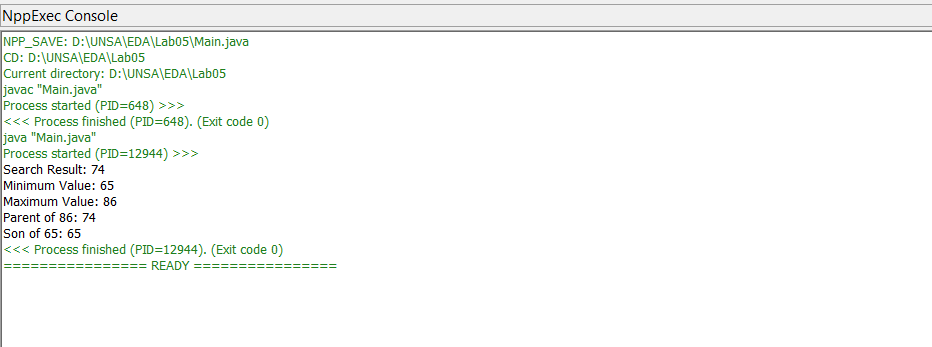
\includegraphics[width=1\textwidth, keepaspectratio]{img/ejemain.png}
    \caption{Ejecución}
  \end{figure}
  
%%%%%%%%%%%%%%%%%%%%

  \section{Recomensaciones}
  \begin{itemize}
    \item Se recomienda utilizar la clase AVLTree en aplicaciones donde se requiera un almacenamiento eficiente de datos que necesiten operaciones de inserción, búsqueda y eliminación frecuentes.
    \item Es importante entender y considerar los principios del balanceo en árboles AVL al realizar modificaciones en el código o adaptarlo a necesidades específicas, para garantizar que el árbol se mantenga balanceado en todo momento.
    \item Se sugiere realizar pruebas exhaustivas con diferentes conjuntos de datos y situaciones límite para evaluar el rendimiento y la robustez de la implementación del árbol AVL.
    \item Para un mejor seguimiento y comprensión del funcionamiento del árbol AVL, se recomienda utilizar herramientas de visualización que permitan observar el proceso de balanceo y la estructura del árbol en diferentes etapas.
    \item Mantener una buena documentación del código, incluyendo comentarios claros y explicativos, facilitará el mantenimiento y la colaboración en proyectos que utilicen la clase AVLTree.
  \end{itemize}

%%%%%%%%%%%%%%%%%%%%

  \section{Conclusiones}
  \begin{itemize}
    \item La utilización de rotaciones simples y dobles permitió mantener el equilibrio del árbol AVL durante las operaciones de inserción y eliminación, garantizando así su eficiencia en términos de tiempo.
    \item La función de búsqueda implementada en el árbol AVL demostró su capacidad para encontrar nodos con rapidez, incluso en árboles de gran tamaño, gracias al balanceo automático que ofrece esta estructura.
    \item La visualización y comprensión de los conceptos relacionados con árboles AVL se vieron facilitadas mediante la representación gráfica de estos árboles, lo que ayudó en el proceso de desarrollo y depuración del código.
    \item En general, la experiencia de trabajar con árboles AVL ha sido educativa y valiosa para comprender en profundidad la importancia de las estructuras de datos balanceadas en la programación.
  \end{itemize}

%%%%%%%%%%%%%%%%%%%%
	\newpage
	\subsection{\textcolor{red}{Rúbrica para el contenido del Informe y demostración}}
	\begin{itemize}			
		\item El alumno debe marcar o dejar en blanco en celdas de la columna \textbf{Checklist} si cumplio con el ítem correspondiente.
		\item Si un alumno supera la fecha de entrega,  su calificación será sobre la nota mínima aprobada, siempre y cuando cumpla con todos lo items.
		\item El alumno debe autocalificarse en la columna \textbf{Estudiante} de acuerdo a la siguiente tabla:
	
		\begin{table}[ht]
			\caption{Niveles de desempeño}
			\begin{center}
			\begin{tabular}{ccccc}
    			\hline
    			 & \multicolumn{4}{c}{Nivel}\\
    			\cline{1-5}
    			\textbf{Puntos} & Insatisfactorio 25\%& En Proceso 50\% & Satisfactorio 75\% & Sobresaliente 100\%\\
    			\textbf{2.0}&0.5&1.0&1.5&2.0\\
    			\textbf{4.0}&1.0&2.0&3.0&4.0\\
    		\hline
			\end{tabular}
		\end{center}
	\end{table}	
	

	\end{itemize}

 
	
	\begin{table}[H]
		\caption{Rúbrica para contenido del Informe y demostración}
		\setlength{\tabcolsep}{0.5em} % for the horizontal padding
		{\renewcommand{\arraystretch}{1.5}% for the vertical padding
		%\begin{center}
		\begin{tabular}{|p{2.7cm}|p{7cm}|x{1.3cm}|p{1.2cm}|p{1.5cm}|p{1.1cm}|}
			\hline
    		\multicolumn{2}{|c|}{Contenido y demostración} & Puntos & Checklist & Estudiante & Profesor\\
			\hline
			\textbf{1. GitHub} & Hay enlace URL activo del directorio para el  laboratorio hacia su repositorio GitHub con código fuente terminado y fácil de revisar. &2 &X &2 & \\ 
			\hline
			\textbf{2. Commits} &  Hay capturas de pantalla de los commits más importantes con sus explicaciones detalladas. (El profesor puede preguntar para refrendar calificación). &4 &X &4 & \\ 
			\hline 
			\textbf{3. Código fuente} &  Hay porciones de código fuente importantes con numeración y explicaciones detalladas de sus funciones. &2 &X &2 & \\ 
			\hline 
			\textbf{4. Ejecución} & Se incluyen ejecuciones/pruebas del código fuente  explicadas gradualmente. &2 &X &2 & \\ 
			\hline			
			\textbf{5. Pregunta} & Se responde con completitud a la pregunta formulada en la tarea.  (El profesor puede preguntar para refrendar calificación).  &2 &X &2 & \\ 
			\hline	
			\textbf{6. Fechas} & Las fechas de modificación del código fuente estan dentro de los plazos de fecha de entrega establecidos. &2 &X &2 & \\ 
			\hline 
			\textbf{7. Ortografía} & El documento no muestra errores ortográficos. &2 &X &2 & \\ 
			\hline 
			\textbf{8. Madurez} & El Informe muestra de manera general una evolución de la madurez del código fuente,  explicaciones puntuales pero precisas y un acabado impecable.   (El profesor puede preguntar para refrendar calificación).  &4 &X &4 & \\ 
			\hline
			\multicolumn{2}{|c|}{\textbf{Total}} &20 & &20 & \\ 
			\hline
		\end{tabular}
		%\end{center}
		%\label{tab:multicol}
		}
	\end{table}


%%%%%%%%%%%%%%%%%%%%%%%%%%%%%%%%%%%%%%%%%%%%%%%%%%%%%%%%%%%%%%%%%%%
	
  \newpage
  \section{Referencias}
  \begin{itemize}
    \item \url{https://www.w3schools.com/java/}
    \item \url{https://www.eclipse.org/downloads/packages/release/2022-03/r/eclipse-ide-enterprise-java-and-web-developers}
    \item \url{https://docs.oracle.com/javase/7/docs/api/java/util/List.html}
    \item \url{https://docs.oracle.com/javase/tutorial/java/generics/types.html}
    \item \url{https://www.baeldung.com/java-avl-trees}
  \end{itemize}

%%%%%%%%%%%%%%%%%%%% 
%\clearpage
%\bibliographystyle{apalike}
%\bibliographystyle{IEEEtranN}
%\bibliography{bibliography}
			
\end{document}
